\documentclass[a4paper,12pt]{article}
\usepackage[utf8]{inputenc}
\usepackage[T2A]{fontenc}
\usepackage{amsmath}
\usepackage{hyperref}
\hypersetup{colorlinks=true}
\usepackage{colortbl}
\usepackage{graphicx}
\usepackage{float}
\usepackage{gensymb}

\pagecolor[rgb]{1,.98,.9}

\title{U{\degree}OS: Distributed ledger data management protocol.}
\author{}

\begin{document}

\maketitle

\begin{abstract}

The concept of a cryptographically protected and distributed transaction ledger has demonstrated its efficiency in a series of projects. The fourth industrial revolution sets a new level of standards for decentralized protocols. The U{\degree}OS project’s approach to the distributed ledger is filtered through the lens of the management of an ever-increasing sea of data produced by a digital society. The protocol architecture aims to correspond with this management  goal, using the Delegated Proof of Importance (DPoI) consensus algorithm. DPoI is a high-performance energy effective, network growth inducing algorithm that rewards network participants for the system's economy enhancing operations. Delegated Proof of Importance is an upgrade to the existing blockchain solutions that integrate the concepts of the Delegated Proof of Stake (DPoS) and the Network Theory. The system protocol is designed in accordance with business and end-user requirements such as privacy, transparency, and smooth volatility, which is achieved due to adaptive emissions proportionate to both network activity growth and the volume of the network itself, according to Metcalfe's law \cite{Metcalfe}.

% Концепция распределенного реестра транзакций защищенного криптографией продемонстрировала свою эффективность. Четвертая промышленная революция задает новый уровень требований к децентрализованным протоколам. Проект U{\degree}OS смотрит на задачи распределенного реестра через призму потребностей управления увеличивающемся массивом данных, создаваемых в результате экономической деятельности в цифровом обществе.  Архитектура протокола стремиться соответствовать этой задаче, используя алгоритм консенсуса Делегированное доказательство значимости (Delegated Proof of Importance, DPoI). DPoI - высокопроизводительный, энергоэффективный и стимулирующий развитие сети алгоритм, вознаграждающий участников сети за операции, являющуюся положительной для экономики системы. Делегированное доказательство значимости развивает существующие блокчейн решения, объединяя концепции  Делегированного доказательства доли (Delegated Proof of Stake, DPoS) и Теории сетей. Протокол системы спроектирован с учетом требований бизнеса и рядовых пользователей, таких, как приватность, аудируемость, мягкая волатильность, достигаемая за счет динамической эмиссии пропорциональной росту активности сети, опираясь на Закон Меткалфа.. \cite{Metcalfe}.
\end{abstract}

\section{Introduction}

Recent years have marked an unprecedented growth in the interest in blockchain technologies. So far, this interest has primarily been seen in the form of distributed payment networks. These networks are decentralized and enable fast low-cost transactions avoiding middlemen. Although the general economic pros and cons of blockchain-based networks are subject to rigorous examination, within this paper, we would like to consider the technical aspects of blockchain consensus algorithms.

The blockchain consensus algorithm is a mechanism that allows the network nodes to reach consensus about the contents of a distributed ledger. The consensus algorithm is the very basis of any blockchain network, which also noticeably determines its technical characteristics.

% Последние годы были отмечены необычайным ростом интереса к технологии блокчейн, при этом основным ее применением пока было создание распределенных платежных сетей. Такие сети являются децентрализованными и позволяют осуществлять быстрые и недорогие транзакции без посредников. Хотя экономические достоинства и недостатки платежных сетей, основанных на блокчейне, заслуживают отдельного рассмотрения в рамках данной бумаги мы планируем подробнее остановиться на технических особенности работы алгоритмов консенсуса в блокчейне.
% 
% Алгоритм консенсуса в блокчейне – это механизм, с помощью которого, в условиях отсутствия централизованного ведения журнала транзакций (реестра) одним субъектом, узлы сети могут достичь консенсуса о содержимом реестра. Именно алгоритм консенсуса является фундаментом любой блокчейн сети, в значительной степени определяющим ее технические особенности.

\subsection{Previous Work}

The problem of a distributed consensus for networks with potentially fraudulent participants (the Byzantine Generals' Problem) was stated long before the creation of blockchain, in 1982. \cite{Lamport} Since then, an array of different solutions have been developed \cite{Castro}. However, the first solution that did not rely on a trusted third party, was the Proof-of-Work (PoW) algorithm, described in Satoshi Nakamoto's article. \cite{satoshi} Despite its advantages, PoW inherently has a number of shortcomings, namely scalability and performance problems \cite{Croman}, security \cite{Eyal}, progressive centralization of the networks around the largest mining pools \cite{Buterin}, and most importantly, the need to use vast volumes of real resources, such as electricity and computing power to generate every block \cite{Bentov}. 

% Задача распределенного консенсуса для сетей, в которых узлы могут быть злоумышленниками (т.н. задача византийских генералов), впервые была сформулирована задолго до появления блокчейна - в 1982 г. \cite{Lamport} С тех пор был разработан целый ряд различных вариантов ее решения \cite{Castro}, однако применительно к блокчейнам первым вариантом решения проблемы стал изложенный в статье Сатоши Накамото \cite{satoshi} алгоритм Proof-of-Work (PoW, доказательство работы). Несмотря на свои преимущества PoW характеризуется рядом недостатков: проблемы с масштабируемостью и производительностью \cite{Croman}, безопасностью \cite{Eyal}, постепенная централизация сети в руках крупнейших майнинг-пулов \cite{Buterin}, и самое важное - необходимость использования значительного объема реальных ресурсов (электроэнергии и вычислительной техники) для генерации каждого \cite{Bentov}.

By now, the computing resources needed for hashing blocks in Bitcoin, are tremendous and far exceed the computing power of the world’s greatest supercomputers. Energy use for mining is comparable to the power consumption of some countries and it continues to grow \cite{energy}. In 2012, in order to mitigate these shortcomings, the PPCoin (now known as PeerCoin)  cryptocurrency became the first to utilize an alternative consensus algorithm, Proof-of-Stake (PoS) \cite{Ppcoin}. In PoS consensus networks, the probability of creating a new block depends on the volume of tokens in a participant’s account. PoS also turns out to have several drawbacks and in its current state, according to a number of experts, cannot serve as an adequate replacement to PoW \cite{Demeester}, \cite{Poelstra}. One of the major weaknesses of PoS is that it additionally motivates users to concentrate all funds in one place or with one user, which leads to centralization of the network. The next iteration of PoS was introduced as the Delegated Proof-of-Stake (DPoS) \cite{dantheman}. Here network members are divided into two groups: members who delegate the authority to create blocks and validate transactions, and validators (producers). This partition provides better scalability and efficiency. Nevertheless, in DPoS there still remains the problem of motivation for a participant to use their assets actively instead of accumulating them, and that has a negative impact on the growth and governability of the network. The Proof-of-Importance consensus algorithm (PoI), was first introduced in the NEM cryptocurrency \cite{nem}. PoI incentivizes network participants' activity. The major departure from PoS is that block generation probability and reward distribution depends not only on the volume of a user's deposits but also on the participant's activity rate and reputation. Thus, the algorithm motivates users to be more active by participating in  more transactions and contributing to the network growth. Despite all its merits, POI has some shortcomings in efficiency. 

% На сегодня вычислительные ресурсы, расходуемые на хеширование блоков в биткоине, огромны и намного превышают мощности крупнейших суперкомпьютеров, а расход энергии на майнинг сопоставим с потреблением электроэнергии целых стран и продолжает расти \cite{energy}.
% Для устранения данных недостатков был придуман альтернативный алгоритм консенсуса - Proof-of-Stake (PoS, доказательство доли), впервые реализованный в 2012 году в криптовалюте PPCoin (сейчас известна под названием PeerCoin) \cite{Ppcoin}. В сетях с консенсусом PoS вероятность сформировать следующий блок зависит от объема токенов на депозите участника сети. Данный алгоритм также обладает рядом недостатков и, по мнению ряда экспертов, в текущем виде не является адекватной заменой PoW \cite{Demeester} \cite{Poelstra}. Одним из важнейших недостатков PoS является то, что он дает дополнительную мотивацию к накоплению средств в одних руках, что способствует централизации сети.
% Развитием PoS стал алгоритм консенсуса Delegated Proof-of-Stake (DPoS, делегированное доказательство доли) \cite{dantheman}. Разделение участников сети на делегирующих и валидирующих (делегатов) обеспечивает лучшую масштабируемость и производительность. Однако в DPoS сохраняется проблема мотивации участников сети к консолидации токенов, вместо их активного использования, что отрицательно сказывается на росте и управляемости сети.
% Для стимулирвоания активности участников сети был спроектирован алгоритм консенсуса Proof-of-importance (PoI, доказательство значимости), используемый в блокчейне NEM \cite{nem}. Ключевое отличие от PoS протоколов состоит в том, что при выборе валидатора блока учитывается не только баланс токенов акаунта, но и транзакционная активность участника. Таким образом, алгоритм мотивирует пользователей быть активными, совершая транзакции и поощряя участие в развитии сети. Несмотря на свои достоинства PoI не лишен недостатков связанных с производительностью. 

\subsection{Project goal}

The major goal of U{\degree}OS is to create a distributed ledger data management protocol with effective power redistribution within the system, which motivates users to participate actively in network development and prevents centralization. Modern blockchain solutions have problems with scalability, security and efficiency, and to solve those problems, U{\degree}OS Protocol introduces the DPoI (Delegated Proof of Importance) Consensus Algorithm. This consensus algorithm combines the advantages of DPoS and PoI and implements a new feature of delegating validation rights to a limited number of accounts in order to achieve high levels of efficiency and scalability within the network, accounting for transaction activity of the protocol members, and leading to its further development.

% Цель U{\degree}OS – создание протокола управления распределенным реестром с эффективным перераспределением влияния в системе, поощряющего пользователей принимать активное участие в развитии сети и препятствующего централизации. Для решения существующих в современных блокчейн решениях проблем с масштабируемостью, производительностью и безопасностью в протоколе U{\degree}OS реализован алгоритм достижения консенсуса DPoI (Delegated Proof of Importance). Алгоритм сочетает в себе достоинства DPoS и PoI, обладая преимуществами оных, реализует возможность делегирования права валидации блоков ограниченному количеству аккаунтов для достижения высокой производительности и масштабируемости сети, учитывая транзакционную активность участников протокола, способствуя ее развитию. 

\section{U{\degree}OS Protocol Consensus Algorithm Operating Principle}

The U{\degree}OS consensus algorithm (Delegated Proof-of-Importance, DPoI) is based on the EOS core consensus algorithm. In addition to the client's stake amount, our algorithm also considers the client's transactional activity. In U{\degree}OS Protocol, all of the participants have the option of delegating the right to validate blocks to a limited number of accounts. To prevent activity imitation or fraud between several affiliated accounts, the transaction graph is partitioned into clusters utilizing the SCAN algorithm  \cite{SCAN}. In general, the working principle of the U{\degree}OS Protocol Consensus Algorithm can be explained as follows.

% Алгоритм консенсуса U{\degree}OS базируется на алгоритме Делегированное доказательство значимости (Delegated Proof of Importance, DPoI), основанном на изменённом ядре EOS, учитывая дополнительно к доли владения узла его транзакционную активность. 
% В протоколе U{\degree}OS всем аккаунта сети доступна возможность делегировать право валидировать блоки ограниченному кругу аккаунтов.
% Для борьбы с имитацией активности между несколькими аффилированными аккаунтами используется разбиение транзакционного графа на кластеры с помощью алгоритма SCAN. В общих чертах принцип работы алгоритма консенсуса протокола U{\degree}OS можно представить следующим образом:

\subsection{Importance index Calculation}

Importance index, which is used in voting, and could be interpreted as an importance rating of an account \textit{i} is calculated as follows: 

% Индекс значимости эккаунта вычисляется следующим образом:
\begin{equation}
    \label{importance_rating}
    r_i = (1 - \omega_a - \omega_s) v_i + \omega_a \pi_i + \omega_s \sigma_i
\end{equation}


Here $v_i$ is the stake volume index, $\pi_i$ is the finance activity index calculated with the NCDawareRank algorithm, $\sigma_i$ if the social network activity index, $\omega_a$ and $\omega_s$ is the weight coefficients. 

% Здесь $v_i$ – индекс доли владения, $\pi_i$ – индекс активности, полученный с помощью алгоритма NCDAwareRank, $\omega$ — весовой коэффициент.

Stake volume index is based on the amount of tokens owned by the account, and represents balance relation to the total amount of tokens in the system. Thus, an account with non-zero balance has non-zero importance index. Activity index depends on transaction history of the account. Activity index is calculated only for accounts with the balance exceeding the $A_0$ threshold. This value is not fixed and is determined by committee members. When calculating the account activity index only transactions with the amount of tokens higher than $T_0$ are taken into account. That value is also determined by the committee. Hidden transactions are not included. Activity index depends on transactions, creation time of which lays in some time interval. The duration of this interval is $W$ blocks. Contribution of every transaction decreases exponentially.

% Индекс доли владения определяется количеством токенов, принадлежащих эккаунту, и представляет собой отношение баланса эккаунта к общему количеству токенов в системе. Таким образом, у любого эккаунта с ненулевым балансом будет ненулевой индекс значимости. Индекс активности зависит от истории транзакций, связанных с данным эккаунтом. Индекс активности вычисляется не для всех эккаунтов, а только для тех, баланс которых на момент вычисления индекса превышает некоторый порог $A_0$. Это значение не является фиксированным, и определяется участниками комитета. Также при вычислении инекса активности учитываются не все транзакции, а только те, в которых сумма передаваемых токенов превышает порог $T_0$, который также определяется комитетом. Скрытые транзакции не учитываются при вычислении индекса активности. Учитываются транзакции не за все время, но только те, которые попадают во временное окно продолжительностью $W$ блоков. Вклад каждой каждой транзакции уменьшается со временем экспоненциально.


\subsection{NCDAwareRank Algorithm}

Activity Index is calculated according to the NCDawareRank algorithm using the following recurrent relation: 

% Индекс активности в соответствии с алгоритмом NCDAwareRank вычисляется с помощью следующего рекуррентного соотношения:

\begin{equation}
    \label{recurrent_formula_for_ncdawarerank}
    \boldsymbol{\pi}^{(i+1)} = ( \eta \boldsymbol{O} + \mu \boldsymbol{M} + ( 1 - \eta - \mu ) \boldsymbol{E} ) \boldsymbol{\pi}^{(i)}
\end{equation}

Here $\pi^{(i)}$ is a vector of account importance indexes values. The vector is normalized, i.e. the sum of its elements is 1. $\boldsymbol{O}$ is the outlink matrix, $\boldsymbol{M}$ is the interlevel proximity matrix. See the definitions of the matrices below. $\eta$ and $\mu$ are weight coefficients that determine contributions of the $\boldsymbol{O}$ and $\boldsymbol{M}$ matrices. Their sum must be less than 1. $\boldsymbol{E}$ is the teleportation matrix added to ensure the series is convergent. This is defined as follows:

% $\pi^{(i)}$ -- вектор, каждый элемент которого -- рейтинг значимости эккаунта. Вектор нормированный, сумма его элементов равна 1.
% $\boldsymbol{O}$ -- outlink-матрица, $\boldsymbol{M}$ – матрица межуровневой близости. Об определении этих матриц см. ниже.
% $\eta$ и $\mu$ – весовые коэффициенты, определяющие вклад матриц $\boldsymbol{O}$ и $\boldsymbol{M}$. Их сумма должна быть меньше единицы.
% $\boldsymbol{E}$ -- матрица телепортации, добавленная для обеспечения сходимости ряда. Она определяется так:

$$
\boldsymbol{E}=\frac{1}{N}\boldsymbol{e}
$$

where \textit{N} is the number of accounts and $\boldsymbol{e}$ is the matrix in which all the elements are equal to 1, the calculation continues until for some i the following condition is fulfilled: 

% где N -- количество эккаунтов, и $\boldsymbol{e}$ -- матрица, все элементы которой равны 1.
% Вычисления продолжаются, пока при некотором i не будет выполнено условие:

$$
norm(\boldsymbol{\pi}^{(i+1)}-\boldsymbol{\pi}^{(i)})<\varepsilon
$$

Here \textit{norm()} is the vector norm defined as the sum of its elements, $\varepsilon$ is the predetermined calculation accuracy. As an initial approximation, $\pi_0$, a vector with all the elements equal to $\frac{1}{N}$ can be used.

% Здесь norm() - это норма вектора, определенная как сумма его элементов, $\varepsilon$ — заранее заданная точность вычислений. 
% В качестве начального приближения, $\pi_0$, может быть использован вектор, все элементы которого равны $\frac{1}{N}$.

\subsection{Outlink matrix calculation}

The outlink matrix $O$ is calculated as follows: First the weight matrix is calculated:

% Outlink-матрица $O$ вычисляется следующим образом. Сначала вычисляется матрица весов:

$$
w_{ij}=\sum_{k|i \to j, {h_k \ge H_0} \land {h_k \le H_0+W}} \theta ( a_k - T_0 ) \theta ( s_i - A_0 ) \theta ( s_j - A_0 ) a_k \exp{(lnK [\frac{h_k}{D}])}
$$

where $a_k$ is the sum of transaction \textit{k}, $h_k$ is the transaction depth (the block order number from the current point, also known as a block height),  $K$ and $D$ are transaction contribution decrease parameters, that define how much the contribution of each transaction decreases over time. The purpose of these parameters is that over every $D$ number of blocks, created after the given transaction, the transaction contribution decreases by $w'=Kw$. The sum is taken over all the transactions of a deposit from account \textit{i} to account \textit{j}, depth of which lays between $H_0$ and $H_0+W$. $H_0$ and $W$ are parameters, its values are equal $H_0=2419200$ and $W=1000$ currently in the testnet. So, only transactions from time gap, duration of which is $W$ blocks, contribute to activity index.


% Здесь $a_k$ – сумма k-й транзакции, $h_k$ – глубина  k-й транзакции (порядковый номер блока, отсчитанный от текущего момента), $K$ и  $D$ — параметры, определяющие, насколько уменьшается вклад каждой транзакции со временем. Смысл этих параметров в том, что каждые $D$ блоков, созданных после определенной транзакции, ее вклад уменьшается как $w'=Kw$.

% Суммирование ведется по всем транзакциям, перемещающим некоторую сумму с эккаунта i на эккаунт j, глубина которых лежит в промежутке между $H_0$ и $H_0+W$. Здесь $H_0$ и $W$ - параметры, для тестнета используются значения $H_0=2419200$ (что соответствует 28 дням при продолжительности блока в 1 секунду) и $W=1000$. Таким образом, при вычисления индекса активности учитывается только транзакции, попадающие в окно шириной $W$ блоков, последний блок которого отстоит от текущего блока на $H_0$.


$$
\hat{o}_{ij} = \begin{cases}
 w_{ji}-w_{ij}
 & \text{if $w_{ji}-w_{ij} > 0$,}\\
 0 & \text{otherwise.}
\end{cases}
$$

Then the matrix that was obtained  is normalized so that the sum of elements in every column is equal to 1.

% Далее, полученная матрица нормируется таким образом, что сумма элементов в каждом столбце была равна единице. 

$$
o_{ij} = \begin{cases}
 \frac{\hat{o}_{ij}} {\sum\limits_{k} \hat{o}_{kj}}
 & \text{if $\sum\limits_{k} \hat{o}_{kj}> 0$,}\\
 0 & \text{otherwise}
\end{cases} 
$$

\subsection{Interlevel proximity matrix calculation}

Let W is a set of all the accounts taken into the Importance Index calculation; W is a set divided into disjoint subsets $A_i$ called NCD-blocks (Nearly Completely Departed). See the SCAN algorithm description for details. For the given “account u”, “$G_u$” is the set of all the accounts, for which the according member of outlink matrix is greater than zero: $o_{uv} > 0$. Then the set of proximal “accounts u” is defined as follows: 

% Множество всех аккаунтов W, участвующих в расчете индекса значимости, разбивается на непересекающиеся подмножества $A_i$, называемые NCD-блоками (NCD – nearly completely departed). О принципе разбиения см. описание алгоритма SCAN. 

%Для данного эккаунта u рассмотрим множество всех эккаунтов $G_u$, такое, что для любого эккаунта $v \in G_u$ соответствующий член outlink-матрицы больше нуля: $o_{uv} > 0$. Множество ближних эккаунтов u тогда определяется следующим образом:

$$
\chi_u = \bigcup_{v \in \{u\} \cup G_u} A_{(v)}
$$

The interlevel proximity matrix is defined as follows:

% Матрица межуровневой близости определяется тогда так:

$$
M_{vu}=\begin{cases}
 \frac{1}{N_u |A_{(v)}|}
 & \text{if $v \in \chi_u$ ,}\\
 0 & \text{otherwise.}
\end{cases}
$$

Where $N_u$ is the number of NCD-blocks in $\chi_u$.

% Здесь $N_u$ означает число NCD-блоков в $\chi_u$.

\subsection{SCAN algorithm based graph partitioning into clusters}

An indirected graph $W = \{V, E\}$ has every vertex representing a client, and every edge representing a non-zero element of the outlink matrix. The structure of the vertex $v$ is the set of all the adjacent vertices:

% Построим ненаправленный граф $W = \{V, E\}$, в котором каждая вершина соответствует эккаунту, и каждое ребро – ненулевому элементу outlink-матрицы.
% Структурой данной вершины v назовем множество всех соседних вершин:

$$
\Gamma(v)=\{w \in V|(v,w) \in E\} \cup \{v\}
$$

The structural similarity of two vertices can be defined as follows:

% Структурным сходством двух вершин назовем следующую величину:

$$
\sigma(v,w)=\frac{ |\Gamma(v) \cap \Gamma(w)|}{\sqrt{|\Gamma(v)||\Gamma(w)|}}
$$

The vertex $\varepsilon$-neighborhood is a set of vertices for which

% $\varepsilon$-окружением вершины назовем множество вершин такое, что

$$
N_{\varepsilon}(v) = \{ w \in \Gamma(v) | \sigma(v,w) \ge \varepsilon \}
$$

The \textit{CORE} is a vertex for which the number of elements in the $\varepsilon$-neighborhood is more than $\mu$.

% Ядром назовем вершину, у которой число элементов в $\varepsilon$-окружении больше некоторого порога $\mu$.

$$
CORE_{\varepsilon,\mu}(v) \Leftrightarrow |N_{\varepsilon} (v)| \ge \mu
$$

Vertex $w$ is directly structurally reachable from vertex $v$ if

% Вершина w находится в прямой структурной доступности от вершины v, если

$$
DirREACH(v,w) \Leftrightarrow CORE_{\varepsilon,\mu}(v) \vee w \in N_{\varepsilon}(v)
$$

Vertex $w$ is structurally reachable from vertex $v$ if

% Вершина w находится в структурной доступности от вершины v, если

$$
REACH(v,w) \Leftrightarrow \exists v_1,...v_n \in V \forall i \in \{1,...n-1\}DirREACH(v_i,v_{i+1})
$$

Vertex $v$ is structurally connected with vertex $w$ if

% Вершина v структурно соединена с вершиной w, если

$$
CONNECT(v,w) \Leftrightarrow \exists u \in V REACH(u,v) \vee REACH(u,w)
$$

A cluster is a subset of vertices structurally connected to each other. It is possible to show that every vertex can only belong to one cluster. A vertex can also belong to no cluster; in this case it can either be a hub if there are vertices belonging to two different clusters in its environment, otherwise it is an independent vertex.

% Подмножество вершин, каждая из которых структурно соединена совсем остальными, называется кластером. Можно показать, что каждая вершина может принадлежать только одному кластеру. Также вершина может не принадлежать ни к одному из кластеров, в этом случае она называется значимым узлом, если среди соседей этой вершины есть такие, которые принадлежат к двум разным кластерам, и отдельно стоящей вершиной в противном случае.

\begin{figure}[h]
      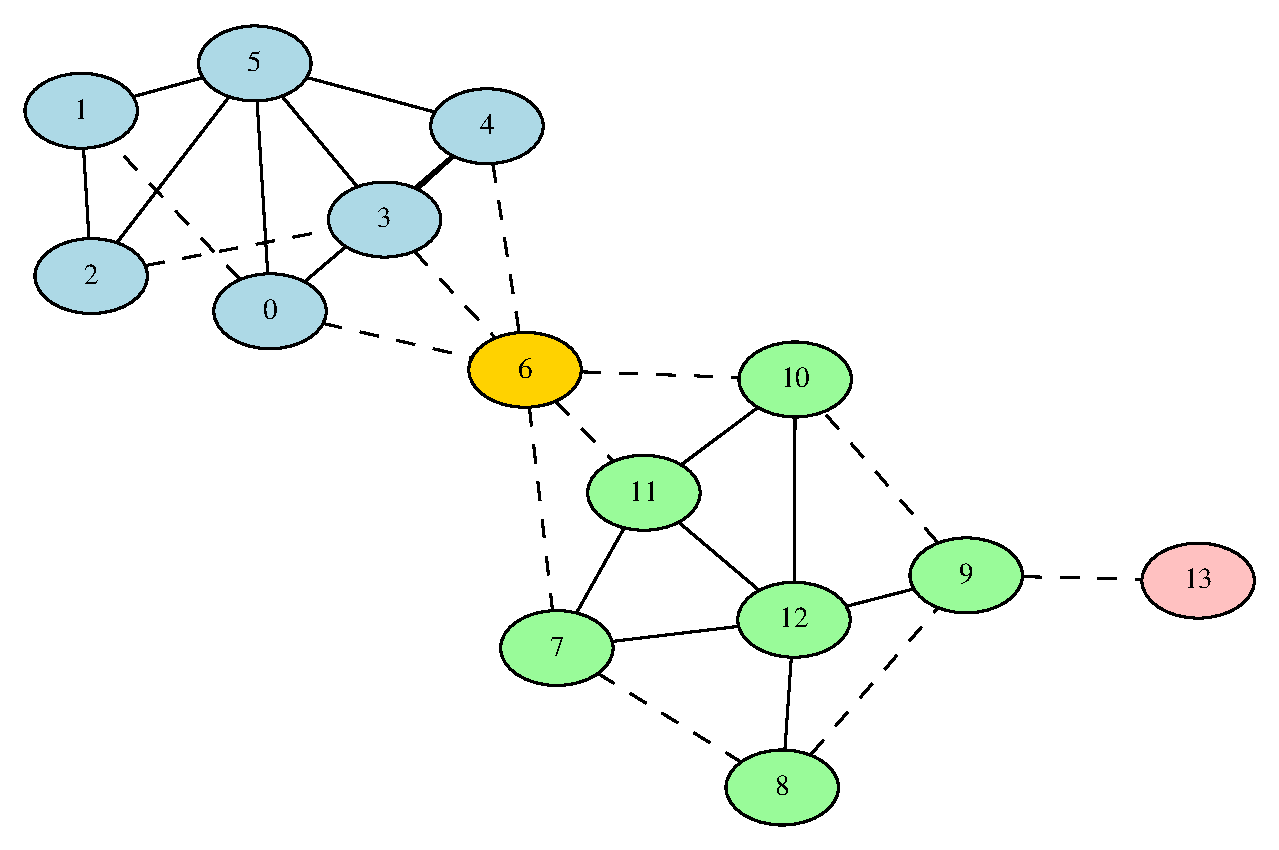
\includegraphics[width=1\linewidth]{pictures/clustering_example.eps}
      \caption{SCAN algorythm applying example. Parameters $\varepsilon=0.7$ and $\mu=4$ were used.}
      \label{fig:sigmoida}
\end{figure}


\subsection{Social network activity index}

U{\degree}OS blockchain is integrated with social network. Every account may have social relations with any other account and may have some content belonging to it. Accounts and content objects with relations between them form a graph. Every account and content object obtains rate depending on involving into social relations. We denote this rate as social network activity index. It is contrubute to importance index, as defined in the formula \ref{importance_rating}.

Social index calculation is based on following data:

The matrix $\boldsymbol{V}$ contains all information about upvotes:
$$
V_{ik} = \begin{cases}
 e^{(ln K)[h/H]}
 & \text{if the account $k$ upvoted the content $i$ at the height $h$,}\\
 0 & \text{otherwise.}
\end{cases}
$$

The matrix $\boldsymbol{P}$ contains all information about content owners:
$$
P_{ik} = \begin{cases}
 1
 & \text{if the content $k$ belongs to the account $i$,}\\
 0 & \text{otherwise.}
\end{cases}
$$

The matrix $\boldsymbol{R}$ contains all information about reposts:
$$
R_{ik} = \begin{cases}
 1 & \text{if the content $i$ is a repost of the account $k$,}\\
 -1 & \text{if $i=k$ and the content $i$ is a repost,}\\
 0 & \text{otherwise.}
\end{cases}
$$

Besides these matrices, calculations are based on the stack vector $\boldsymbol{s}$ and a weight vector $\boldsymbol{w}$, containing priority values for every account. 

Based on these data structures, we may caclulate social activity vectors for accounts $\boldsymbol{\sigma^a}$ and content $\boldsymbol{\sigma^c}$. These vectors are normalized to 1:

$$
\sum_i{\sigma^a_i} = 1, \sum_i{\sigma^c_i} = 1
$$



We may obtain now the matrix $\boldsymbol{V'}$:

$$
\boldsymbol{V'} = ( \boldsymbol{I} + \boldsymbol{R} ) \boldsymbol{V}
$$

And the matrix $\boldsymbol{U}:$

$$
\hat{U}_{ik} = max_n(P_{in} V'_{nk})
$$

To provide effective decaying weights with time, we add a special ``hidden'' account $h$, which accepts upvotes from every account:

$$
\forall i \ne h \hat{U}_{hi} = 1,
\forall i\hat{U}_{ih} = 0
$$

$$
U_{ik} = \begin{cases}
 \frac{\hat{U}_{ik}} {\sum_n{\hat{U}_{nk}}} & \text{if $\sum_n{\hat{U}_{nk}}>0$} \\
 0 & \text{otherwise.}
\end{cases}
$$

We may now use the PageRank algorithm to calculate $\boldsymbol{\sigma^a}$:

$$
\boldsymbol{\hat{\sigma}^a}^{(n+1)} = (\alpha \boldsymbol{U} + (1 - \alpha) \boldsymbol{T})\boldsymbol{ \hat{\sigma}^a}^{(n)}
$$

The teleportation matrix $\boldsymbol{T}$ contains information about initial weights of accounts:

$$
\boldsymbol{T} = ((1 - \beta - \gamma) \boldsymbol{e} + \beta \boldsymbol{w} + \gamma \boldsymbol{s}) \boldsymbol{e}^T
$$

Here $\beta$ and $\gamma$ are koefficients with values between 0 and 1, $\boldsymbol{e}$ is unit vector.

Further, we should subtract contribution of stack from the rating vector, because social index of an account should not depend on this account's stack:

$$
\boldsymbol{\dot{\sigma}^a} = \frac{1}{1 - (1-\alpha) \gamma}(\boldsymbol{\hat{\sigma}^a} - (1 - \alpha) \gamma \boldsymbol{s})
$$

Finally, we must remove the from rating vector the ``hidden'' account. This operation changes norm of the rating vector, so we must normalize it to 1:

$$
\sigma^a_i = \frac{\dot{\sigma}^a_i}{\sum_{j \ne h} \dot{\sigma}^a_j}, i \ne h
$$






Based on $\boldsymbol{\sigma^a}$, we may obtain $\boldsymbol{\sigma^c}$:

$$
\boldsymbol{\sigma^c} = \boldsymbol{V'}\boldsymbol{\sigma^a}
$$

\subsection{Resistance to attacks}

Following mitigations are used in the project, in order to reduce the risk of attacks.

\begin{itemize}
  \item Only incoming transfers contribute to importance index, it makes obtaining score from existing accounts more difficult.
  \item There are stake threshold for accounts, participating in importance index calculation, and amount threshold fot transfers. It makes attacks more expensive for attackers.
  \item Using NCDAwareRank instead of PageRank makes the system more resistant to splitting account attacks. This algorythm gives preference to accounts, tightly integrated to common network.
  \item Koefficients $\omega_a$ and $\omega_s$ have relatively small values, it makes contribution of activity index and social index to total importance index significantly less than stake contribution.
  \item Using decaying weights makes effect of any fraud activity temporary. Stopping fraud activity causes quick decreasing obtained score.
\end{itemize}


\subsection{The use of importance index in the system}

Importance index is used for two purposes:

First, it defines the amount of new tokens which every account receives in case the emission is positive. 

Second, importance index defines the account’s weight during the voting. The voting allows the delegation  of certain powers within the system to a limited number of the accounts. 

Producers who own nodes that produce and verify blocks are selected by voting.

Members of the committee are also selected by voting. The committee can vote on blockchain settings, such as the fee amount for a transaction, producer node reward and so on. 

% Индекс значимости используется для двух целей. 
% 
% Во-первых, при очередной эмиссии индекс значимости определяет долю новых токенов, которыю получит каждый эккаунт.
% 
% Во-вторых, индекс значимости определяет вес данного эккаунта при голосовании. Голосование позволяет делегировать определенные полномочия в системе ограниченному количеству эккаунтов.
% 
% Путем голосования выбираются узлы, которые осуществляют формирование блоков. 
% 
% Также путем голосования выбираются члены комитета. Комитет может голосованием менять параметры блокчейна, такие, как размер комиссии за трансфер, вознаграждение producer-нодам и т.п.


\section{The Protocol Token}

The amount of transactions processed directly depends on the available computing power provided by network members. To allocate the resources efficiently and to avoid spam attacks, a fee in the protocol core cryptographic token is levied on the operations within the U{\degree}OS network. The protocol allows a user to make token transfer transactions between the network members and launch system smart contracts, e.g. multi-signature, account registration, user tokens creation and so on.

% Объём обрабатываемых операций блокчейн протоколом напрямую зависит от доступной вычислительной мощности, предоставленной участниками сети. Для эффективного распределения ресурсов системы и предотвращения spam атак, при совершении операций в сети U{\degree}OS с пользователей удерживается комиссия системы в криптографическом токене протокола.. 
% Протокол позволяет совершать транзакции трансфера токена между аккаунтами участников сети и вызова умных контрактов системы, таких как мульти-подпись, регистрация аккаунтов, создание пользовательских токенов и т.д.. 

\section{Emission}

Emission amount at launch is 1,000,000,000 protocol tokens, distributed to the original network accounts to start the protocol. The U{\degree}OS project implements adaptive emission. The emission volume is calculated regularly once, in a certain time interval, $t_0, t_1, ... t_i$, where $t_{i+1} = t_i + T$. The volume of emission depends on the network activity growth in the preceding time period $T$.

% Стартовая эмиссия составляет 1000000000 токенов протокола, распространяется по изначальным аккаунтам сети для запуска функционирования протокола.   
% В проекте U{\degree}OS используется динамическая эмиссия. Эмиссия производится регулярно, в моменты времени $t_0, t_1, ... t_i$, где $t_{i+1} = t_i + T$. Объем эмиссии зависит от роста активности сети за предыдущий период T.

\subsection{Calculating network activity for a period of time}

To begin, we calculate the matrix of weights according to the formula:

% Вычислим сперва матрицу весов по следующей формуле:

$$
w_{ij}(t_n)=\sum_{k|i \to j, t_k \in [t_{n-1}, t_n]}a_k
$$

Here $a_k$  is the amount in k-th transaction, $t_k$  the time at which k-th transaction was created. Summation is performed for all the transactions transferring any amount from account $i$ to account $j$ and created at the time frame from $t_{n-1}$ to $t_n$. 

In fact, each matrix element $w_{ij}$ represents a weight of connection between account $i$ and account $j$ in a given time frame. Next we need to calculate the matrix of connections $l$: 

% Здесь $a_k$ – сумма k-й транзакции, $t_k$ – время создания k-й транзакции. Суммирование ведется по всем транзакциям, перемещающим некоторую сумму с эккаунта i на эккаунт j, созданным за период от $t_{n-1}$ до $t_n$.
% 
% Каждый элемент матрицы $w_{ij}$ представляет собой вес связи между эккаунтом $i$ и $j$ за данный период.
% 
% Вычислим теперь матрицу связей $l$:

$$
l_{ij}(t_n) = \begin{cases}
 1
 & \text{if $w_{ji}(t_n)-w_{ij}(t_n) > 0$,}\\
 0 & \text{otherwise.}
\end{cases}
$$

We calculate the activity in a given time frame as:

% Активность за период мы будем вычислять так:

$$
A(t_n) = \sum_{i,j} l_{ij}(t_n)
$$

In this way, activity is calculated as a number of connections between active accounts in a set timeframe. 

% Таким образом, активность вычисляется как количество связей между активными эккаунтами за данный период.

\subsection{Emission value calculation}

Emission value depends on network activity growth.

$E_T$ value is defined as follows, and it is the target value of emission. It defines the upper bound of the aggregate amount of the emission, that is achievable with the following activity value $A$:

% Объем эмиссии зависит от роста активности сети.
% 
% Определим величину $E_T$, которую назовем целевой величиной эмиссии. Она задает верхнюю границу совокупной величины эмиссии, достижимой при данном значении активности A.

$$
\Delta A(t_n) = A(t_n) - A_{max}(t_{n-1})
$$

$$
E_T(t_n) = \begin{cases}
 E_T(t_{n-1}) + K_E \Delta A(t_n),
 & \text{when $\Delta A(t_n) > 0$,}\\
 E_T(t_{n-1}) & \text{otherwise}
\end{cases}
$$

Here $K_E$ is a coefficient which defines the maximum value of the emission with activity increased by 1. $A_{max}(t_{n-1})$ is the previous maximum value since the system launch:

% Здесь $K_E$ - коэффициент, определяющий максимальную величину эмиссии при увеличении активности на единицу, $A_{max}(t_{n-1})$ - максимальное предыдущее значение активности с момента запуска системы:

$$
    A_{max}(t_{n-1}) = max \Big ( A(t_i), t_i \in [t_0, t_{n-1}] \Big )
$$

Emission value, which is issued at a certain time $t_n$, is defined by formula:

% Величина эмиссии, выпускаемая в момент времени t, вычисляется по формуле:

$$
    E(t_n) = \lambda S(t_{n-1}) f \Big( \kappa \frac {E_T(t_n) - E_S(t_{n-1})}{\lambda S(t_{n-1})} \Big)
$$

Here $\lambda$ is the marginal growth of the token amount in the system S per one emission. It is defined through $L$, which specifies the marginal growth $S$ in a year, expressed as a percentage:

% Здесь $\lambda$ -- предельный рост количества токенов в системе S за один выпуск эмиссии. Он определяется из параметра L, который задает предельный рост S в год (выраженный в процентах):

$$
    \lambda = (1 + \frac{L}{100})^{1/N}-1
$$

Here $N$ is the number of emission issues per year.

% Здесь N - количество выпусков эмиссии в год.

$f(x)$ - sigmoidal function (Fig \ref{fig:sigmoida}). In the present implementation of the algorithm a hyperbolic tangent is used as this function. 

% $f(x)$ - сигмоидальная функция (Рис. \ref{fig:sigmoida}). В имеющейся реализации алогитма в качестве этой функции используется гиперболический тангенс.

$\kappa$ is a coefficient between 0 to 1 and it defines the speed at which a full emission approaches the target emission $E_T$ if the activity level remains the same over the long term.

% $\kappa$ -- коэффициент от 0 до 1, определяющий скорость, с которой полная эмиссия приближается к целевой эмиссии $E_T$, в случае, если активность остается но одном уровне на протяжении длительного срока.

Initial values of both $E_T$ and $E_S$ are zero:

%Начальные значения $E_T$ и $E_S$ равны нулю:

$$
E_T(t_0)=0, E_S(t_0)=0
$$


\begin{figure}[h]
      \includegraphics[width=1\linewidth]{pictures/sigmoida.eps}
      \caption{Sigmoidal function}
      \label{fig:sigmoida}
\end{figure}


\addcontentsline{toc}{section}{Bibliography}
\begin{thebibliography}{99}
 \bibitem{Metcalfe} Metcalfe, B. (2013). Metcalfe's law after 40 years of ethernet. Computer, 46(12), 26-31. URL: http://ieeexplore.ieee.org/abstract/document/6636305/
 \bibitem{Lamport} Lamport, L., Shostak, R., Pease, M. (1982). The Byzantine generals problem. ACM Transactions on Programming Languages and Systems (TOPLAS), 4(3), 382-401. URL: https://www.microsoft.com/en-us/research/uploads/prod/2016/12/The-Byzantine-Generals-Problem.pdf
 \bibitem{Castro} Castro, M., Liskov, B. (2002). Practical Byzantine fault tolerance and proactive recovery. ACM Transactions on Computer Systems (TOCS), 20(4), 398-461. URL: https://dl.acm.org/citation.cfm?doid=571637.571640
 \bibitem{satoshi} Nakamoto, S. (2008). Bitcoin: A peer-to-peer electronic cash system. URL: https://bitcoin.org/bitcoin.pdf
 \bibitem{Croman} Croman, K. et al. (2016). On scaling decentralized blockchains. In International Conference on Financial Cryptography and Data Security (pp. 106-125). Springer, Berlin, Heidelberg. URL: http://www.comp.nus.edu.sg/~prateeks/papers/Bitcoin-scaling.pdf
 \bibitem{Eyal} Eyal, I., Sirer, E. G. (2014). Majority is not enough: Bitcoin mining is vulnerable. In International conference on financial cryptography and data security (pp. 436-454). Springer, Berlin, Heidelberg. URL: https://arxiv.org/pdf/1311.0243.pdf
 \bibitem{energy} Bitcoin Energy Consumption Index. digiconomist.net. URL: https://digiconomist.net/bitcoin-energy-consumption
 \bibitem{Buterin} Buterin, V. (2014). Mining Pool Centralization at Crisis Levels. URL: https://bitcoinmagazine.com/articles/mining-pool-centralization-crisis-levels-1389302892/
 \bibitem{Bentov} Bentov, I., Gabizon, A., Mizrahi, A. (2016). Cryptocurrencies without proof of work. In International Conference on Financial Cryptography and Data Security (pp. 142-157). Springer, Berlin, Heidelberg. URL: https://link.springer.com/chapter/10.1007/978-3-662-53357-4\_10/
 \bibitem{Ppcoin} King, S., Nadal, S. (2012). Ppcoin: Peer-to-peer crypto-currency with proof-of-stake. URL: https://peercoin.net/assets/paper/peercoin-paper.pdf
 \bibitem{Demeester} Demeester, T. (2017). Critique of Buterin’s A Proof of Stake Design Philosophy. URL: https://medium.com/@tuurdemeester/critique-of-buterins-a-proof-of-stake-design-philosophy-49fc9ebb36c6
 \bibitem{Poelstra} Poelstra, A. (2014). Distributed consensus from proof of stake is impossible. URL: https://download.wpsoftware.net/bitcoin/old-pos.pdf
 \bibitem{dantheman} Dantheman. (2017). DPOS Consensus Algorithm - The Missing White Paper. URL: https://steemit.com/dpos/@dantheman/dpos-consensus-algorithm-this-missing-white-paper
 \bibitem{nem} NEM Technical Reference. Version 1.2.1. February 23, 2018 URL: https://nem.io/wp-content/themes/nem/files/NEM\_techRef.pdf
\bibitem{SCAN} Xiaowei Xu et al. (2007). SCAN: A Structural Clustering Algorithm for Networks. URL: http://www1.se.cuhk.edu.hk/~hcheng/seg5010/slides/p824-xu.pdf
\end{thebibliography}

\section {Appendix 1 Glossary of Terms}

\textbf{U{\degree}OS consensus algorithm (Delegated Proof-of-Importance, DPoI)}

The consensus algorithm, which is based on a calculation of the importance index of an account, which in turn depends on Stake Volume Index and Activity index

\textbf{Importance index}

The importance index of an account is calculated as a function of Stake Volume Index and Activity index

\textbf{Account}

An entity represented by a tuple of pairs of keys (public + private), which is registered in a blockchain by an individual.

\textbf{Producer}

Accounts with the right to verify blocks. They must have a node.

\textbf{Node}

A P2P network node, which performs all the calculations in blockchain. A node belonging to a producer account (producer node), produces blocks.

\tableofcontents

\end{document}
